%\documentclass[12pt,a4paper]{article}
%\usepackage[utf8]{inputenc}
%\usepackage[english]{babel}
%\usepackage{amsmath}
%\usepackage{amsfonts}
%\usepackage{amssymb}
%\usepackage{graphicx}
%\usepackage[left=3cm,right=3cm,top=2.5cm,bottom=4cm]{geometry}
%\author{Ari-Pekka Honkanen}
%\title{Notes on Magnetism}
%\linespread{1.3}

%\begin{document}
%\maketitle
\section{Pauli equation}
A suitable starting point to investigate magnetism in atomic systems is the Pauli equation, which describes the dynamics of a non-relativistic spin-1/2 particle in an electromagnetic field. A single electron with the mass $m$ and the charge $-e$ the standard form of the time-independent equation is
\begin{equation}
\left[\frac{(\mathbf{p} + e \mathbf{A})^2}{2m} + \frac{e \hbar}{m} \mathbf{s} \cdot \mathbf{B} - e \phi \right] | \psi \rangle = E | \psi \rangle,
\end{equation}
where $\phi$ is the electric scalar potential, $\mathbf{A}$ is the (unquantized) vector potential, the magnetic field $B=\nabla \times \mathbf{A}$ and $\mathbf{s} = (s_x,s_y,s_z)$ are the components of the (unitless) spin-1/2 operator. Quite often $s_i$ are given in terms of Pauli matrices:
\begin{equation}
s_x = \frac{1}{2}\left( \begin{matrix}
0 & 1 \\
1 & 0 
\end{matrix} \right)
\qquad 
s_y = \frac{1}{2}\left( \begin{matrix}
0 & -i \\
i & 0 
\end{matrix} \right) 
\qquad
s_z = \frac{1}{2}\left( \begin{matrix}
1 & 0 \\
0 & 1 
\end{matrix} \right).
\end{equation}
In such a representation the state $| \psi \rangle$ is represented by a two-component spinor
\begin{equation}
| \psi \rangle = \left( \begin{matrix} \psi_+ \\ \psi_- \end{matrix} \right) =
\psi_+ |\uparrow \rangle + \psi_- | \downarrow \rangle
.
\end{equation}

Let us consider an ion with $N$ electrons. The Pauli equation now reads
\begin{equation}
\sum_{i=1}^N \left[\frac{(\mathbf{p}_i + e \mathbf{A}_i)^2}{2m} + \frac{e \hbar}{m} \mathbf{s}_i \cdot \mathbf{B}_i - e \phi_i \right] | \psi \rangle = E | \psi \rangle,
\end{equation}
where
\begin{equation}
\phi_i =\frac{1}{4\pi \epsilon_0} \left(\frac{Z_n e}{ |\mathbf{r}_i|} - \frac{1}{2} \sum_{j \neq i} \frac{e}{|\mathbf{r}_i - \mathbf{r}_j|} \right)
\end{equation}
is the electrostatic potential due to the nuclear charge and other electrons\footnote{Factor of $\frac{1}{2}$ is added to avoid double counting}.
$\mathbf{r}_i$ is the position vector of $i$th electron. Assuming that $\mathbf{A}_i$ are in Coulomb gauge \emph{i.e.} $\nabla \cdot \mathbf{A}_i = 0$, we may expand\footnote{Note that $\mathbf{p}_i$ and $\mathbf{A}_i$ are operators that do not commute. The obtained result was derived using a test function.}
\begin{equation}
(\mathbf{p}_i + e \mathbf{A}_i)^2 = \mathbf{p}_i^2 
+ \underbrace{e \mathbf{p}_i \cdot\mathbf{A}_i}_{=0}
+ 2 e \mathbf{A}_i \cdot \mathbf{p}_i
+ e^2 \mathbf{A}_i^2 = \mathbf{p}_i^2 
+ 2 e \mathbf{A}_i \cdot \mathbf{p}_i
+ e^2 \mathbf{A}_i^2.
\end{equation}
Therefore the total Hamiltonian can be written as $\hat{H} = \hat{H}_0 + \hat{H}_M$, where 
\begin{equation}
\hat{H}_0 = \sum_i \frac{\mathbf{p}_i^2}{2 m} - e \phi_i,
\end{equation}
is the electronic part without magnetic interactions and 
\begin{equation}\label{eq:H_magnetic}
\hat{H}_M = \sum_i \frac{e}{m}\mathbf{A}_i\cdot\mathbf{p}_i + \frac{e^2 \mathbf{A}_i^2}{2 m} + \frac{e \hbar}{m} \mathbf{s}_i \cdot \mathbf{B}_i,
\end{equation}
describes the contribution of the magnetic field.

\section{Magnetic energy}
Omitting the spin-orbit interaction, consider an ion which is put into a homogeneous magnetic field $\mathbf{B}_i = \mathbf{B}_0$. In this case the vector potential can be chosen so that 
\begin{equation}
\mathbf{A}_i = -\frac{1}{2}\mathbf{r}_i \times \mathbf{B}_0
\end{equation}
Therefore\footnote{Again, the derivation using a test function.}
\begin{equation}
\mathbf{A}_i\cdot\mathbf{p}_i = 
-\frac{1}{2} \left(\mathbf{r}_i\times\mathbf{B}_0\right)\cdot \mathbf{p}_i
= \frac{1}{2} \mathbf{B}_0 \cdot  \left(\mathbf{r}_i\times\mathbf{p}_i\right)
= \frac{\hbar}{2} \mathbf{B}_0 \cdot  \mathbf{l}_i, 
\end{equation}
where in the last step we have defined a unitless orbital angular momentum operator $\hbar \mathbf{l}_i = \mathbf{r}_i\times\mathbf{p}_i$. Without the loss of generality, we may choose $z$-axis to be parallel with $\mathbf{B}_0$. Thus
\begin{equation}
\mathbf{A}_i\cdot\mathbf{p}_i = \frac{\hbar B_0}{2} l_{z,i},
\end{equation}
where $l_{z,i}$ is the $z$-component of $\mathbf{l}_i$. Similarly
\begin{equation}
\mathbf{A}_i^2 = \frac{1}{4} (\mathbf{r}_i \times \mathbf{B}_0)^2 =
\frac{1}{4} (y_iB_0\hat{\mathbf{x}} - x_iB_0\hat{\mathbf{y}} )^2 = \frac{B_0^2}{4}(x_i^2+y_i^2)
\end{equation}
Substituting the derived expressions for $\mathbf{A}_i\cdot\mathbf{p}_i$ and $\mathbf{A}_i^2$, and $\mathbf{s}_i\cdot\mathbf{B}_i = B_0 s_{z,i}$ into Eq.~\eqref{eq:H_magnetic}, we obtain
\begin{equation}
\hat{H}_M = \sum_i \frac{e \hbar B_0}{2m}l_{z,i} + \frac{e^2 B_0^2}{8 m} (x_i^2 + y_i^2) + 
\frac{e \hbar B_0}{m} s_{z,i}.
\end{equation}
We may simplify the result by defining the Bohr magneton 
\begin{equation}
\mu_B = \frac{e \hbar}{2 m} = 5.788 \cdot 10^{-5}\ \frac{\mathrm{eV}}{\mathrm{T}} 
= 9.274 \cdot 10^{-24}\ \frac{\mathrm{J}}{\mathrm{T}} .
\end{equation}
Thus
\begin{equation}
\hat{H}_M = \mu_B B_0 (L_z + 2 S_z) + \frac{e^2 B_0^2}{8 m} \sum_i (x_i^2 + y_i^2),
\end{equation}
where $L_z = \sum_i l_{z,i}$ and $S_z = \sum_i s_{z,i}$ are the $z$-components of the total orbital angular momentum and spin angular momentum operators $\mathbf{L}$ and $\mathbf{S}$, respectively.


Since magnetic energy is rather small compared to the energy of an unperturbed atom, we may obtain it by using the perturbation theory. Up to the first order the magnetic energy is
\begin{equation}\label{eq:E_magnetic}
\Delta E_M = \mu_B B_0 \langle \psi | L_z + 2 S_z | \psi \rangle 
+ \frac{e^2 B_0^2}{8 m}\sum_i \langle \psi | x_i^2 + y_i^2 | \psi \rangle
\end{equation} 
If we deal with ions with a one electron short being half filled shell, or molecules that do not have an axis of symmetry parallel to the magnetic field, we have to include also the second order contribution
\begin{equation}
\sum_{\psi' \neq \psi} \frac{|\langle \psi | L_z + 2 S_z | \psi' \rangle|^2}{E_\psi - E_{\psi'}},
\end{equation}
where the sum goes over all the exited states. This term is the source of so called \emph{Van Vleck paramagnetism} which will not be consider further in these notes.

\section{Magnetization and thermodynamics}
The magnetization $\mathbf{M}$ connects the magnetic flux density $\mathbf{B}$ and the magnetic field strength $\mathbf{H}$ as follows
\begin{equation}
\mathbf{B}= \mu_0(\mathbf{H}+\mathbf{M}),
\end{equation}
where $\mu_0 = 4\pi \cdot 10^{-7}$~H/m is the permeability of the vacuum. The quantity which is the measure of "magnetisability" of the material as a response to an external field is known as the magnetic susceptibility $\chi$, which can be defined as\footnote{Here $\chi$ is a scalar quantity but in general it can be a tensor $\chi_{ij} = \partial M_i/\partial H_j$}
\begin{equation}
\chi = \frac{\partial M}{\partial H}
\end{equation}
We now take a brief tour into thermodynamics because it is a necessary tool for calculating the magnetic properties. The partition function $Z$ is defined as
\begin{equation}
Z =  \sum_{n} e^{-E_n/k_B T}.
\end{equation} 
Since the magnetic energy is given by $E=-\mathbf{m}\cdot\mathbf{B}=-m_zB_0$, we find that
\begin{equation}
\frac{\partial Z}{\partial B_0} = \sum_{n} -\frac{1}{k_B T} e^{-E_n/k_B T} \frac{\partial E_n}{\partial B_0} =  \frac{1}{k_B T} \sum_{n} m_{z,n} e^{-E_n/k_B T}.
\end{equation}
Thus the magnetization of the system is
\begin{equation}
M = \frac{\langle m_z\rangle}{V} = \frac{1}{V}\frac{k_B T}{Z} \frac{\partial Z}{\partial B_0}
\end{equation}
Since the Helmholtz energy $A = - k_B T \ln Z$, the former can be simplified
to
\begin{equation}
M = \frac{\langle m_z\rangle}{V} = - \frac{1}{V} \frac{\partial A}{\partial B_0}.
\end{equation}
Thus the magnetic susceptibility can be obtain from $A$ as follows
\begin{equation}
\chi = \frac{\partial M}{\partial H} =  - \frac{1}{V} \frac{\partial^2 A}{\partial H \partial B_0}.
\end{equation}
If $\chi$ is small, then $\mathbf{B} \approx \mu_0 \mathbf{H}$ and we get
\begin{equation}
\chi = \frac{\partial M}{\partial H} =  - \frac{\mu_0}{V} \frac{\partial^2 A}{\partial B_0^2}
\end{equation}

\section{Diamagnetism}
Consider an ion which contains only filled shells. For such an ion $L^2|\psi\rangle = S^2|\psi\rangle = 0$ and thus the magnetic energy \eqref{eq:E_magnetic} becomes
\begin{equation}
\Delta E_M = \frac{e^2 B_0^2}{8 m}\sum_i \langle \psi | x_i^2 + y_i^2 | \psi \rangle.
\end{equation}
In low temperatures, only the ground state of the system is populated: the Helmholtz energy of $N$ ions is simply $A = N\Delta E_M$. Therefore the susceptibility of such ions in the volume $V$ is
\begin{equation}
\chi = -\frac{\mu_0 N}{V} \frac{\partial^2 \Delta E_M}{\partial B_0^2}
= -\frac{N}{V} \frac{\mu_0 e^2}{4 m}\sum_i \langle \psi | x_i^2 + y_i^2 | \psi \rangle.
\end{equation}
Since the shells are filled, we may assume that the ion is spherically symmetric, thus $\langle \psi | x_i^2| \psi \rangle = \langle \psi | y_i^2 | \psi \rangle = \frac{1}{3} \langle \psi | r_i^2| \psi \rangle $. Furthermore, we may write $\sum_i \langle \psi | r_i^2| \psi \rangle = Z_{e} r^2$, where $Z_{e}$ is the number of electrons and $r$ is the effective ionic radius. Thus the susceptibility becomes
\begin{equation}
\chi_{dia} =  -\frac{N}{V} \frac{\mu_0  e^2}{12 m} Z_{e} r^2.
\end{equation}
The susceptibility caused by this term is negative, so it goes against the applied magnetic field. Thus it is fitting to call the macroscopic magnetic response \emph{diamagnetic}\footnote{\emph{dia} = against, across}. More specifically, the derived term is known as the \emph{Larmor diamagnetism}.


\section{Total angular momentum $J$}
Consider a system where orbital and spin angular momenta are decoupled from each other. The states of such a system are consequently the eigenstates of operators $\mathbf{L}^2$, $\mathbf{S}^2$, $L_z$, and  $S_z$. Thus the states can be characterised by the quantum numbers $L$, $S$, $m_L$, and $m_S$  or $|LSm_Lm_S\rangle$. 
However, the situation changes if we add in the spin-orbit interaction. If the interaction strength is weak compared to the Coulomb interaction, we may consider its effect as a small perturbation. Therefore we may still use the $L$ and $S$ as the good quantum numbers. However, the same does not apply to $m_L$ and $m_S$. 

In absence of the spin-orbit coupling, the directions of $\mathbf{L}$ and $\mathbf{S}$ are independent allowing the determination of their $z$-components  simultaneously. On the other hand, introducing the spin-orbit interaction Hamiltonian of the form
\begin{equation}
\hat{H}_{LS} = \Lambda \mathbf{L}\cdot\mathbf{S}
\end{equation}
fixes the angle between $\mathbf{L}$ and $\mathbf{S}$ owing to which the energy eigenstates are no longer eigenstates of $L_z$ and $S_z$. Stated in more mathematical terms, we may write $\mathbf{L} \cdot \mathbf{S} = L_x S_x + L_y S_y + L_z S_z$ since $\mathbf{L}$ and $\mathbf{S}$ commute. Whereas $|LSm_Lm_S\rangle$ is an eigenstate for $L_z$ and $S_z$ operators, it not so for $x$- and $y$-components. Thus the magnetic quantum numbers $m_L$ and $m_S$ are not good quantum numbers for describing the eigenstates of LS-coupled system.


%However, the situation changes if we add in spin-orbit interaction, $\Hat{H}_{\rm SO}$. 
%\begin{align}
%\hat{H} &= \hat{H}_0 + \Hat{H}_{\rm SO}\\
%\Hat{H}_{\rm SO} &= \sum_i\xi_i(r) \mathbf{l}_i \cdot \mathbf{s}_i\\
%\xi(r) &= \frac{\hbar^2}{2m^2c^2r}\frac{\partial U(r)}{\partial r},
%\end{align}
%where $\hat{H}_0$ is the part of the Hamiltonian in which $\mathbf{l}_i$ and $\mathbf{s}_i$ are disconnected.

%Given the radial function $R_{n,l}(\mathbf(r))$ of a single electron state, we define the single electron SOC constant 
%\begin{equation}
%\zeta_{n,l} = \hbar^2\int_0^\infty r^2\mathrm{d}\mathbf{r}~|R_n,l(\mathbf{r})|^2\xi(\mathbf{r})
%\end{equation}
%and in a Coulombic potential
%\begin{equation}
%\zeta_{n,l}  = \frac{e^2\hbar^2}{8\pi\epsilon_0m^2c^2a_0^2}\frac{Z_{\rm eff}^4}{n^3l(l+1)(l+\frac{1}{2})}
%\end{equation}
%which provides a good guideline for when the spin-orbit effect is most significant.

%A useful result due to Condon and Shortley (Mabbs \& Machin: magnetism and transition metal complexes) is that, within a single shell 
%\begin{align}
%E_{\rm SO}  &\equiv \langle LSm_Lm_S|H_{SO}|LSm_Lm_S\rangle = \Lambda \langle LSm_Lm_S|\mathbf{L}\cdot\mathbf{S}|LSm_Lm_S\rangle
%\end{align}

%The constant of proportionality $\Lambda$ is called the \textit{term} spin-orbit coupling (SOC) constant, and is the more directly measurable quantity, but the inferred single electron SOC constant is a property shared with other configurations.

%Since $\mathbf{L}$ and $\mathbf{S}$ commute, we may write $\mathbf{L} \cdot \mathbf{S} = L_x S_x + L_y S_y + L_z S_z$. This is where the problem arises. Whereas $|LSm_Lm_S\rangle$ is an eigenstate for $L_z$ and $S_z$ operators, it not so for $x$- and $y$-components. Thus the magnetic quantum numbers $m_L$ and $m_S$ are not good quantum numbers for describing the eigenstates of LS-coupled system.

To tackle the problem, we define the total angular momentum operator 
\begin{equation}
\mathbf{J} = \mathbf{L} + \mathbf{S}.
\end{equation}
Since $\mathbf{L}$ and  $\mathbf{S}$ commute, also $\mathbf{J}$ commutes with them. This means that an eigenstate of $\mathbf{L}^2$ and $\mathbf{S}^2$ is also an eigenstate of $\mathbf{J}^2$. It can also be shown that such an eigenstate is also an eigenstate of $J_z$ labelled by $m_J$. Since $J_z = L_z + S_z$ it is easy to see that the state $|LSm_Lm_S\rangle$ is also an eigenstate of $J_z$. However, \emph{the converse is not true}. This is illustrated in Figure~\ref{fig:angular_momenta_sums}.

Now since $\mathbf{J}^2 = \mathbf{L}^2 + 2\mathbf{L} \cdot \mathbf{S} + \mathbf{S}^2$, we find that the interaction Hamiltonian $\hat{H}_{LS}$
\begin{equation}
\Lambda \mathbf{L} \cdot \mathbf{S} = \frac{\Lambda}{2}(\mathbf{J}^2-\mathbf{L}^2-\mathbf{S}^2 )
\end{equation}
which is conformant with the earlier argument that for the weak spin-orbit coupling the eigenstates are still the eigenstates of $\mathbf{L}^2$ and $\mathbf{S}^2$. Therefore we arrive at the conclusion that the good quantum numbers describing the LS-coupled system are $J$, $L$, $S$, and $m_J$. 

\begin{figure}
\centering
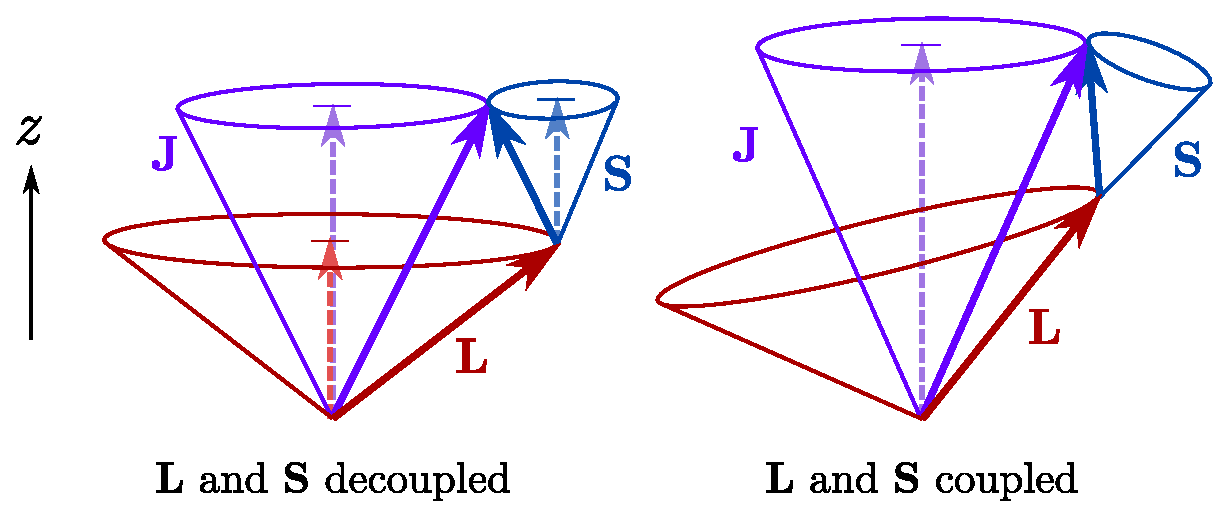
\includegraphics[width=0.8\textwidth]{magnetism/figures/angular_momenta_sums}
\caption{The effect of the LS-coupling to the summation of the angular momenta.\label{fig:angular_momenta_sums}}
\end{figure}

\section{Magnetic moment $\mu_J$ and Land\'{e} g-factor}

\begin{figure}[h!]
\centering
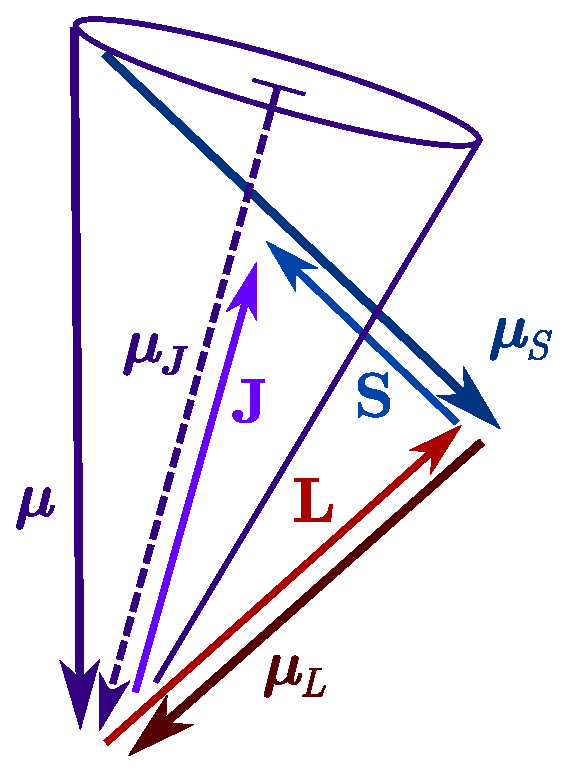
\includegraphics[width=0.3\textwidth]{magnetism/figures/mu_J}
\caption{Summation of the orbital and spin magnetic moments\label{fig:mu_J}}
\end{figure}

What is the magnetic moment associated with the total angular momentum then?
As depicted in Figure~\ref{fig:mu_J}, the total magnetic moment is not parallel with $\mathbf{J}$ since the g-factors of the orbital and spin magnetic moments differ. However, since $\mathbf{L}$ and $\mathbf{S}$ precess around $\mathbf{J}$ so does the total magnetic moment. Therefore it has definitive component $\boldsymbol{\mu}_J$ (anti)parallel to $\mathbf{J}$ and thus we find that the expectation value of the magnetic momentum $\boldsymbol{\mu}$ is 
\begin{equation}
\langle JLSm_J|\boldsymbol{\mu}|JLSm_J\rangle
= \langle JLSm_J|\boldsymbol{\mu}_J|JLSm_J\rangle
\end{equation}
Therefore it also holds that 
\begin{equation}\label{eq:mu_dot_J}
\langle JLSm_J|\boldsymbol{\mu}\cdot\mathbf{J}|JLSm_J\rangle
= \langle JLSm_J|\boldsymbol{\mu}_J\cdot\mathbf{J}|JLSm_J\rangle
\end{equation}
Since $\boldsymbol{\mu}_J \| \mathbf{J}$, we may write
\begin{equation}
\boldsymbol{\mu}_J = - g_J \mu_B \mathbf{J},
\end{equation}
where $g_J$ is the \emph{Land\'{e} g-factor} which can be interpreted as the effective number of Bohr magnetons pointing at the direction of $\mathbf{J}$. Now the right hand side of Eq.~\eqref{eq:mu_dot_J} becomes
\begin{equation}
\langle JLSm_J|\boldsymbol{\mu}_J\cdot\mathbf{J}|JLSm_J\rangle = - g_J \mu_B \langle JLSm_J|\mathbf{J}^2 |JLSm_J\rangle = - g_J \mu_B J(J+1) \label{eq:r_mu_dot_J}
\end{equation}
Similarly, since $\boldsymbol{\mu} = - \mu_B (\mathbf{L} + 2 \mathbf{S}) = - \mu_B (\mathbf{J} + \mathbf{S})$, the left hand side of Eq.~\eqref{eq:mu_dot_J} becomes
\begin{align}
\langle JLSm_J|\boldsymbol{\mu}_J\cdot\mathbf{J}|JLSm_J\rangle &= - \mu_B \langle JLSm_J|\mathbf{J}^2+\mathbf{S}^2+\mathbf{S}\cdot\mathbf{L}|JLSm_J\rangle
\nonumber \\
&= - \mu_B \frac{1}{2} \langle JLSm_J|3 \mathbf{J}^2+ \mathbf{S}^2-  \mathbf{L}^2|JLSm_J\rangle 
\nonumber \\
&= - \mu_B \frac{3J(J+1)+S(S+1)-L(L+1)}{2}, \label{eq:l_mu_dot_J}
\end{align}
where $\mathbf{J}^2 = \mathbf{L}^2 + 2\mathbf{L} \cdot \mathbf{S} + \mathbf{S}^2$ has been used. Thus by combining the Equations~\eqref{eq:r_mu_dot_J} and \eqref{eq:r_mu_dot_J} we find that the Land\'{e} g-factor is
\begin{equation}
g_L = \frac{3}{2} + \frac{S(S+1)-L(L+1)}{2J(J+1)}
\end{equation}
\bibliographystyle{plain}
\bibliography{magnetism/refs}
 
\nocite{ashcroftmermin,blundell_book}

\end{document}
